\chapter{Standard e Concetti base}

\section{Standard}
Ci sono diverse organizzazioni che si occupano di standard:
\begin{itemize}
    \item NIST (\textit{National Institute of Standars and Technology})
    \item ISOC (\textit{Internet Society})
    \item ITU-T (\textit{International Telecommunicatin Union})
    \item ISO (\textit{International Organization for Standardization})
    \begin{itemize}
        \item 27001: documento a cui fare riferimento per costruire un sistema di gestione 
        della sicurezza delle informazioni che possa essere certificato da un ente indipendente 
        \item 27002: non è certificabile, è una raccolta di \textit{best practices} per 
        soddisfarre i requisiti della 27001
    \end{itemize}
\end{itemize}

\section{Reference Monitor Model - RMM}

\begin{figure}[H]
    \centering
    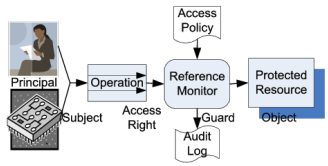
\includegraphics[width=0.75\linewidth]{chapters/2/images/rmm.png}
\end{figure}

Il \textbf{reference monitor} è un \textbf{sistema dotato di una politica di controllo 
degli accessi}. Si occupa di:
\begin{itemize}
    \item \textbf{autenticare chi vuole accedere}
    \item \textbf{autorizzare} o meno le operazioni richieste in base ai permessi 
    \item fare \textbf{audit} $\rightarrow$ tenere un log delle azioni compiute
\end{itemize}

\section{Definizioni}
\begin{itemize}
    \item La \textbf{sicurezza informatica} è l'insieme di strumenti, politiche, linee guida \dots che 
    possono essere utilizzate per proteggere l'ambiente e le risorse dell'organizzazione e 
    degli utenti del cyberspazio 
    \item I \textbf{beni dell'organizzazione e degli utenti} comprendono i dispositivi informatici 
    connessi, personale, infrastrutture e la totalità delle informazioni trasmesse e/o 
    archiviate nel cyberspazio 
    \item Gli \textbf{obiettivi} generali di sicurezza comprendono \textit{disponibilità, integrità e 
    confidenzialità}
    \item \textit{Sottoinsiemi} della sicurezza informatica:
    \begin{itemize} 
        \item \textbf{Sicurezza delle informazioni:} conservazione della CIA delle informazioni 
        \item \textbf{Sicurezza delle reti:} protezione delle reti e del loro servizio da modifiche non 
        autorizzate e garanzia che la rete svolga correttamente le sue funzioni critiche
    \end{itemize}
\end{itemize}

\section{Sfide della sicurezza informatica}

\begin{itemize}
    \item Non è semplice; può avere requisiti semplici ma \textbf{meccanismi di implementazione complessi}
    \item Nello sviluppo di un meccanismo di sicurezza, si deve sempre \textbf{considerare 
    potenziali attacchi}
    \item Le procedure utilizzate per fornire particolari servizi possono essere \textbf{controintuitive 
    poiché complesse}
    \item Bisogna decidere \textbf{dove utilizzare i meccanismi di sicurezza}, sia a livello 
    logico che a livello fisico
    \item I meccanismi di sicurezza in genere coinvolgono \textbf{più di un algoritmo 
    o protocollo}
    \item Una battaglia \textbf{continua} tra attaccante e difensore
\end{itemize}

\section{Principi fondamentali di progettazione della sicurezza}
\begin{itemize}
    \item \textbf{Fail-safe default:} nel caso in cui il sistema vada in default, deve rimanere
    in uno \textit{stato protetto}
    \item \textbf{Economia di meccanismo:} i meccanismi devono essere il più semplice possibile 
    \item \textbf{Mediazione completa:} \textit{tutti} gli accessi devono essere controllati per assicurarsi 
    che siano consentiti; solitamente accade che solo la prima interazione è controllata 
    \item \textbf{Design aperto:} la sicurezza non deve dipendere dalla segretezza della sua progettazione 
    o implementazione
    \item \textbf{Seperazione dei privilegi:} un sistema non dovrebbe concedere l'autorizzazione in base 
    a \textit{una singola} condizione
    \item \textbf{Minimi privilegi:} devono essere concessi il minor numero possibile di privilegi
    ad ogni soggetto; eventuali permessi addizionali devono essere concesso per il tempo minimo possibile
    \item \textbf{Accettabilità psicologica:} i meccanismi di sicurezza non dovrebbero rendere l'accesso 
    ad una risorsa più difficile
    \item \textbf{Isolamento}
    \item \textbf{Incapsulamento}
    \item \textbf{Modularità}
    \item \textbf{Stratificazione (\textit{layering})}
    \item \textbf{Minima sorpresa:} evitare che l'utente si trovi davanti a situazioni inaspettate 
    che potrebbero portarlo a seguire comportamenti scorretti
\end{itemize}

\section{Superificie di attacco}
Una superficie di attacco è costituita dalle \textbf{vulnerabilità raggiungibili e sfruttabili} in 
un sistema, come ad esempio:
\begin{itemize}
    \item porte aperte verso l'esterno
    \item interfacce web
    \item dipendente con accesso a dati sensibili 
    \item \dots
\end{itemize}
$\rightarrow$ è necessario \textbf{ridurre al minimo} la superificie di attacco

\subsection{Categorie di attacco}
\begin{itemize}
    \item Superificie di attacco di \textbf{rete}: sono incluse vulnerabilità del protocollo
    di rete, che possono portare a DoS, interruzione dei collegamenti di comunicazioni ed altri 
    attacchi intrusivi
    \item Superficie di attacco \textbf{software}: vulnerabilità nel codice delle applicazioni; un focus 
    particolare è il software per server web 
    \item Superificie di attacco \textbf{umano}: vulnerabilità create dal personale o da estranei, come 
    \textit{social engeneering}, errore umano o intrusi
\end{itemize}

\section{Albero di attacco}
Un albero di attacco è un modo ti \textbf{rappresentare le possibilità di attacco}, e quindi
di progettare le \textbf{contromisure}.

\section{Tipi di attacco}
\begin{itemize}
    \item \textbf{Passivi:} non alterano le informazioni in transito; lo scopo è ottenere 
    informazioni sui messaggi trasmessi
    \item \textbf{Attivi:} modificano il flusso delle informazioni 
    \begin{itemize}
        \item \textit{Attacco di replay:} l'attaccante osserva le informazioni e le riutilizza 
        in un secondo momento per creare una nuova sessione di comunicazione

        $\rightarrow$ ci si tutela con \textit{numeri casuali} e \textit{timestamp} per, rispettivamente,
        controllare che i messaggi non siano già stati scambiati o che siano ancora validi
        \item \textit{DoS e DDoS}
        \item \dots
    \end{itemize}
\end{itemize}

\section{Implementazione della sicurezza}
Quattro linee d'azione complementari:
\begin{itemize}
    \item \textbf{Prevenzione}
    \item \textbf{Rilevamento}
    \item \textbf{Risposta} in modo da fermare un attacco e prevenire ulteriori danni
    \item \textbf{Ripristino} con sistemi di backup in caso l'integrità dei dati sia compromessa
\end{itemize}























